\subsection*{Multimodal PET/CT Tumour
Segmentation and Prediction of
Progression-Free Survival using a
Full-Scale UNet with Attention}

% \subsection*{Ссылка} \url{https://arxiv.org/abs/2111.03848}
\subsubsection*{Введение}
Опухоли головного мозга и шеи являются пятыми по распространенности 
онкологическими заболеваниями в мире. Сегментация новообразований 
в области головы и шеи и предсказание исхода болезни важны 
для диагностики, лечения и мониторинга заболевания.Ручная сегментация
новообразований, локализованнных в голове и шее является более сложной задачей по 
сравнению с другими частями тела, потому что опухоль показывает похожие 
значения интенсивности с соседними тканями, и человеческому глазу трудно отделить 
больную ткань от здоровой по КТ-изображению. На данный момент комбинация ПЭТ/КТ 
играет ключевую роль в диагностике новообразований. В данной работе
решается задача сегментации опхолей головы и шеи с помощью 
сверточной нейронной сети, а также задача предсказания выживаемости пациентов с помощью 
регресионной модели. \par 
\subsubsection*{Основная идея}
Авторы предлагают \cite{NormRes} производить сегментацию опухолей головы и шеи по ПЭТ/КТ 
изображениям, используя полномасшатбную сеть архитектуры 3D UNet3++ \cite{Unet} с механизмом,
имитирующим когнитивное внимание (attention mechanism).  Предложенная модель, 
NormResSE-UNet3+ была обучена с гибридной функцией потерь, состоящей из Log Cosh Dice и Focal loss. 
Далее, предсказанные карты сегментации дополнительно уточняются с помощью механизма постпроцессинга -
Conditional Random Fields, чтобы уменьшить число ложноположительных ответов 
и улучшить сегментацию границы опухоли. Для решения задачи предсказания 
выживаемости предлагается регресионная модель CoxPH относительной опасности, использующая 
комбинацию клинических, radiomics (признаки, полученные из медицинских изображений с помощью определенных методов) признаков, а также признаков, полученных при глубоком обучении на ПЭТ/КТ-изображениях.
\par
\subsubsection*{Предобработка данных}
Для задачи сегментации была использована трилинейная интерполяция (trilinear interpolation) ПЭТ и КТ-изображений.
Интесивность ПЭТ была нормализована с помощью Z-score, а интенсивность КТ, 
приведена к [-1,1]. \par
Данные для предсказания выживаемости были обработаны с учетом пропущенных значений. Каждый пропущенный признак - 
это функция от существующих признаков. Пропущенные признаки восстанавливаются итеративно
с помощью Lasso регрессии и 5-fold кросс-валидации на клинических, радиомических признаках и признаках, полученных из 3D-UNet.

% \newline

\begin{minipage}{1.0\linewidth}
    \begin{center}
    
    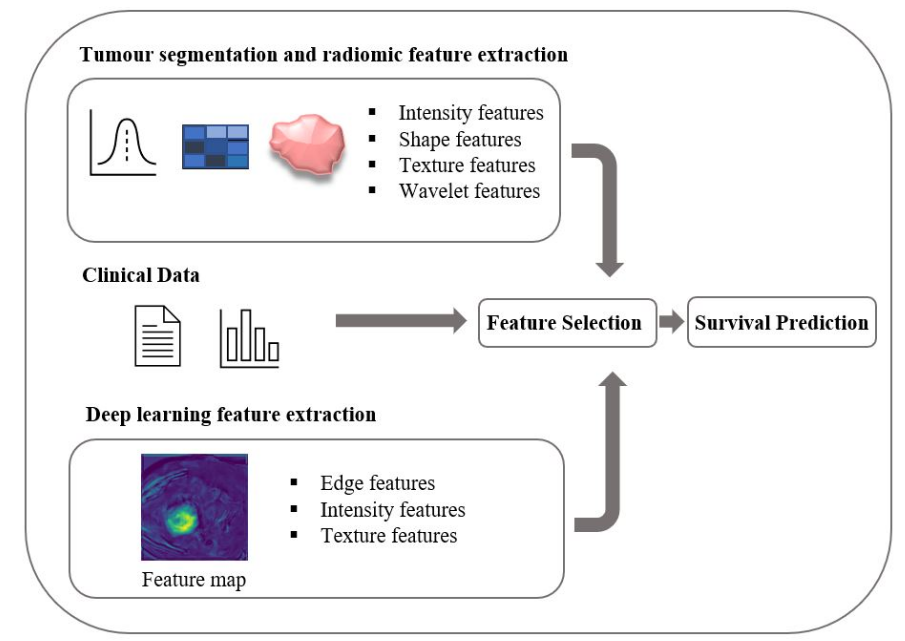
\includegraphics[scale=0.49]{annot6_features.jpg} \\
    \captionof{figure}{\scriptsize{Пайплайн для задачи предсказания выживаемости. Состоит из трех шагов:
    сбор клинических \\ данных, изображений и препроцессинга. Затем, выбираются извлеченные признаки и производится \\
    предсказание выживаемости.}}
\end{center}
\end{minipage}


\subsubsection*{Модель для сегментации}
Архитектура предложенной сети NormResSE-UNet3+: 
\begin{itemize}
    \item На вход подается тензор, размерности 2x144x144x144, состоящий из конкатенации
    ПЭТ и КТ изображений.
    \item Энкодер состоит из residual squeeze-and-excitation блоков, первый блок из которых 
    содержит 24 фильтра. Размерность выхода энкодера 384x3x3x3
    \item Путь декодирования состоит из полномасштабных соединений и модуля, содержащего 
    правильную разметку изорбражений (ground truth).
    \item У декодера одноканальный выход размерности 1х144х144х144
\end{itemize}



\begin{minipage}{1.0\linewidth}
    \begin{center} 
    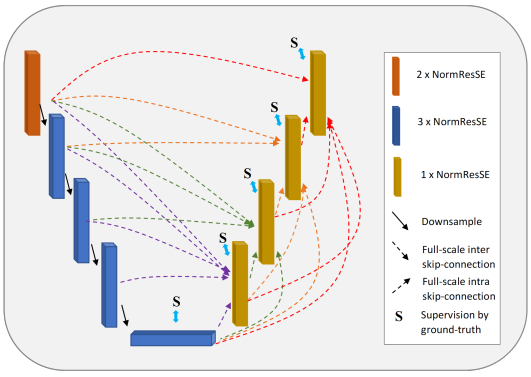
\includegraphics[scale=0.5]{ann6_arch.png}\\
    \captionof{figure}{\scriptsize{Архитектура NormResSE-UNet3+}}
    
    \end{center}

\end{minipage}


% \subsection*{Данные}
Данные были предоставленны организаторами соревнования HECTOR - MICCAI. Всего 
тренировочных примеров - 224 из 5 центров: CHGJ, CHMR, CHUS,CHUP,CHUM.
\par
% \subsection*{Результаты}
Было обучено несколько моделей нейронных сетей для задачи сегментации опухолей головы и шеи. 
Результаты сведены в единую таблицу.



{\small
\captionof{table}{Количественные результаты сегментации}
\begin{tabular}{|l| c| c| c| c|}
    \hline

     Cross-validation fold & \multicolumn{2}{|c|}{NormResSE-UNet3+} & \multicolumn{2}{|c|}{NormResSE-UNet3+ + CRF} \\
    \cline{1-5}
      & DSC & HD &  DSC & HD95 \\

    \hline
    Fold 1 & 0.792 & 3.18 & 0.822 & 3.11\\ \cline{2-5}
    \hline

    Fold 2 & 0.693 & 3.43 & 0.702 & 3.41\\ \cline{2-5}
    \hline
    Fold 3 & 0.728 & 3.32 & 0.749 & 3.29\\ \cline{2-5}
    \hline
    Fold 4 & 0.736 & 3.31 & 0.738 & 3.30\\ \cline{2-5}
    \hline
    Fold 5 & 0.742 & 3.29 & 0.756 & 3.28\\ \cline{2-5}
    \hline
    Ensemble & 0.738 & 3.30 & 0.753 & 3.28\\  \cline{2-5}
    \hline
 
    \hline \hline
    \end{tabular}
}
\\





{\small 

\captionof{table}{Результаты предсказания выживаемости. Предложенная регрессионная модель CoxPH показала 
лучший результат:}
\begin{tabular}{l c}
    
\hline 
    Survival Models   & C-index \\ [0.5ex] 
    \hline\hline 
    CoxPH Regression (clinical) & 0.70 \\
    CoxPH Regression (clinical + PET radiomics) & 0.67 \\
    CoxPH Regression (clinical + CT radiomics)  & 0.68 \\
    CoxPH Regression (clinical + PET/CT radiomics) & 0.72 \\
    CoxPH Regression (clinical + deep learning features) & 0.76 \\
    \textbf{CoxPH Regression (clinical + CT radiomics + deep learning features)} & \textbf{0.82} \\
    Random Survival Regression (clinical) & 0.59 \\
    Random Survival Regression (clinical + PET radiomics) & 0.60 \\
    Random Survival Regression (clinical + CT radiomics) & 0.61 \\
    Random Survival Regression (clinical + PET/CT radiomics) & 0.59 \\
    Random Survival Regression (clinical + CT radiomics + deep learning features) & 0.58 \\
    DeepSurv (clinical) & 0.60 \\
    DeepSurv (clinical + PET radiomics) & 0.68 \\
    DeepSurv (clinical + CT radiomics) & 0.69 \\
    DeepSurv (clinical + PET/CT radiomics) & 0.73 \\
    DeepSurv (clinical + PET/CT radiomics + deep learning features & 0.65) \\ [1ex]
    \hline 
\end{tabular}

}
